\section{Introduction} \label{sec:introduction}
    \IEEEPARstart{R}{espiratory} motion reduces image resolution in \gls{PET} by introducing blurring and mis-alignment artefacts~\cite{Nehmeh2008a}. Unless gated \gls{CT} are available (which themselves increase dose to the patient), to avoid mis-registration due to attenuation mismatches, most existing \gls{MC} methods rely on pair-wise registration of gated \gls{NAC} \gls{PET} volumes~\cite{LungMotionDiaphragmBaiBib, Oliveira2014}. This is a challenging problem due to the low contrast and high noise of these volumes. Other \gls{MC} methods can incorporate, directly, both \gls{MC} and \gls{Mu-Map} estimation into reconstruction, however, these can be computationally expensive~\cite{Bousse2016b}.
    
    In our previous work we investigated the possibility of using a \gls{MM} for respiratory \gls{MC} where the \gls{MM} was derived from \gls{NAC} \gls{PET}. One of the advantages of using a \gls{MM} approach over pair-wise registering the data is that the \gls{MM} approach is more robust to noise in the images. We found that \gls{NAC} \gls{TOF} \gls{PET} was suitable to estimate the motion from gated PET data without inter-respiratory cycle variation~\cite{Whitehead2019ImpactPET}. This work extends the method towards attenuation correction with a single \gls{Mu-Map} (from any position).

% \vspace{-0.5cm}

\section{Methods} \label{sec:methods}
    % \vspace{-0.25cm}
    
    \subsection{XCAT Volume Generation} \label{sec:xcat_volume_generation}
        \gls{XCAT}~\cite{Segars2010} was used to generate $240$ volumes over a \SI{120}{\second} respiratory trace (with inter-respiratory cycle variation) derived from data captured using a \gls{RPM}. The max displacement of \gls{AP} and \gls{SI} motion was set to \SI{1.2}{\centi\metre} and \SI{2.0}{\centi\metre} respectively. Activity concentrations were derived from a static \gls{FDG} patient scan. The \gls{FOV} included the base of the lungs, diaphragm and the top of the liver with a \SI{20}{\milli\metre} diameter spherical lesion placed into the centre of the right lung.
    
    % \vspace{-0.5cm}
    
    \subsection{PET Acquisition Simulation} \label{sec:pet_acquisition_simulation}
        \gls{PET} acquisitions were simulated (and reconstructed) using \gls{STIR}~\cite{Thielemans2012, Nikos2019, Wadhwa2020PETLibrary} through the \gls{SIRF}~\cite{Ovtchinnikov2017} to forward project the data using the geometry of a \gls{GE} Discovery $710$ with a \gls{TOF} resolution of \SI{375}{\pico\second}. This \gls{TOF} resolution is higher than that of the $710$, but is closer to the newer \gls{GE} Signa \gls{PET}/MR system. \gls{TOF} mashing was used to reduce computation time resulting in $13$ \gls{TOF} time bins of size \SI{376.5}{\pico\second}. Attenuation was included using the relevant \glss{Mu-Map} generated by \gls{XCAT}. Scatter and randoms were not taken into account. Multiple noise realisations were generated to simulate an acquisition over \SI{120}{\second}, emulating a standard single bed position acquisition. A respiratory \gls{SS} was generated using \gls{PCA}~\cite{Thielemans2011}. This was used to gate the data into $10$ respiratory bins using displacement gating. For the purpose of the \gls{MM} fitting, \gls{SS} values were ascertained for the post-gated data by taking an average of the \gls{SS} values of the data in each bin.
    
    % \vspace{-0.5cm}
    
    \subsection{Non-Attenuation Corrected Image Reconstruction} \label{sec:non-attenuation_corrected_image_reconstruction}
        Data were reconstructed without \gls{AC} using OSEM with two full iterations and $24$ subsets.~\cite{Hudson1994}.
        Volumes were post-filtered using a Gaussian blur with a kernel size of \SI{6.4}{\milli\metre} full width half maximum.
    
    % \vspace{-0.5cm}
    
    \subsection{Motion Model Estimation} \label{sec:motion_model_estimation}
        The \gls{MM} method, in this work, makes use of \gls{3D} B-spline \glss{CPG} with the corresponding warping operation denoted as $\mathbf{W}(\mathbf{\alpha}_t)$, with $\mathbf{\alpha}_t$ a vector with motion parameters at time $t$ and the breathing surrogate signal $\mathbf{s}$:
    
        % \vspace{-0.25cm}
        
        \begin{equation}
            \forall t \in [1, n_t],\quad \alpha_{n, t} := R_{1, n} s_{1, t} + R_{2, n}
        \end{equation}
        
        % \vspace{-0.025cm}
        
        \noindent where $\alpha_{n, t}$ is the motion parameter $n$ at time point $t$ and $R_{i, n}$ are the model parameters where $i = [1, 2]$. A generalised framework unifying image registration and respiratory \glss{MM} were used to estimate \glss{MM} and \glss{MCI}~\cite{McClelland2017}. Sum of squared differences was used as the similarity measure and bending energy was used as a penalty. The \gls{CPG} spacing and penalty weight were tuned using a grid search.
    
    % \vspace{-0.5cm}
    
    \subsection{Attenuation Map Warping} \label{sec:attenuation_map_warping}
        A \gls{Mu-Map} close to the mean respiratory position was selected from the \glss{Mu-Map} generated by \gls{XCAT}. This \gls{Mu-Map} was then registered (using \gls{NMI}) to the mean position \gls{NAC} \gls{MCI} generated using the \gls{MM}.
        The \gls{MM} was then used to generate \glss{DVF} for the \gls{SS} values of each bin, which were then used to warp the \gls{Mu-Map} from the mean respiratory position to each bin.
    
    % \vspace{-0.5cm}
    
    \subsection{Motion Corrected Image Reconstruction with AC} \label{sec:attenuation_corrected_image_reconstruction}
        Data were re-reconstructed, with \gls{AC}, using the \glss{Mu-Map} from~\Fref{sec:attenuation_map_warping}. The same reconstruction parameters as in~\Fref{sec:attenuation_corrected_image_reconstruction} were used. These data were then either motion corrected using the original \gls{NAC} \gls{MM} or a new \gls{MM} was fit on the \gls{AC} volumes as in~\Fref{sec:motion_model_estimation}.
    
    % \vspace{-0.5cm}
    
    \subsection{Evaluation} \label{sec:evaluation}
        To evaluate the validity of the \gls{MM} results, the \gls{COM} of the lesion, over time, was tracked for both \gls{NAC} and \gls{AC} reconstructions. This was achieved by warping a volume only including the lesion in the reference position, and then computing its \gls{COM}.
        
        In addition to the reconstructions performed in~\Fref{sec:attenuation_corrected_image_reconstruction} data were also reconstructed after simply summing all gates together, using either a sum of all \glss{Mu-Map} (to emulate an average CINE-CT) or one \gls{Mu-Map}, positioned close to the mean respiratory position. This process matches current clinical practice. 
        
        Comparisons used included: A profile over the lesion and \gls{SUV}\textsubscript{max}, \gls{SUV}\textsubscript{median} and \gls{SUV}\textsubscript{peak}. \gls{SUV}\textsubscript{peak} here was defined following \gls{EANM} guidelines~\cite{Boellaard2015FDG2.0}.

% \vspace{-0.5cm}

\section{Results} \label{sec:results}
    \begin{figure}
        \centering
        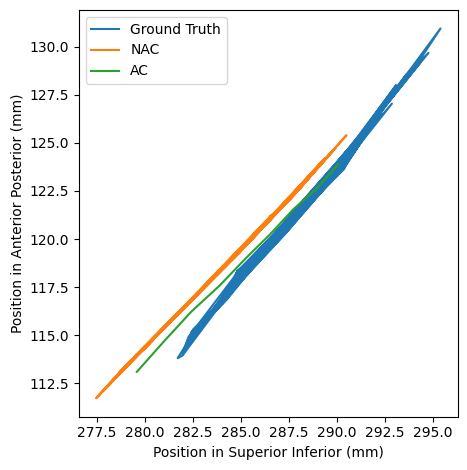
\includegraphics[width=0.75\linewidth]{figures/com.png}
        \captionsetup{singlelinecheck=false, justification=centering}
        \caption{The path of the \gls{COM} of the lesion. Horizontal (respectively vertical) axis corresponds to motion in the \gls{SI} (respectively \gls{AP}). Different curves denote \gls{COM} displacement for  ground truth data, the estimated data from the \gls{NAC} based \gls{MM} and the estimated data from the \gls{AC} based \gls{MM}.}
        \label{fig:com}
    \end{figure}
    
    \gls{COM} results can be seen in~\Fref{fig:com}, the \gls{COM} of both the \gls{NAC} and \gls{AC} matches closely the ground truth \gls{COM}.
    
    \begin{figure}
        % \vspace{-0.5cm}
        \centering
        
        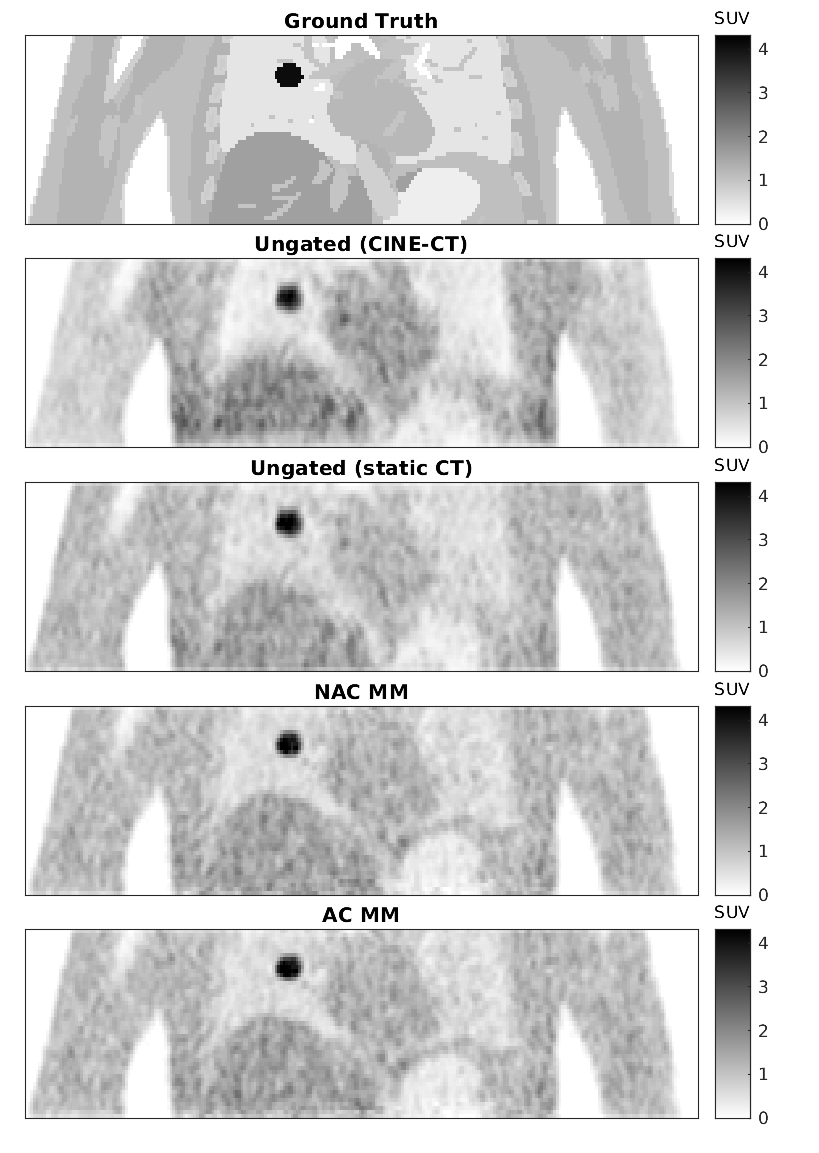
\includegraphics[width=1.0\linewidth]{figures/visual_analysis.png}
        
        % \vspace{-0.6cm}
        
        \captionsetup{singlelinecheck=false, justification=centering}
        \caption{Ground truth and reconstructions using; ungated (CINE-\gls{CT}), ungated (static \gls{CT}), \gls{NAC} \gls{MM}, \gls{AC} \gls{MM}. Colour map ranges are consistent for all images.}
        
        \label{fig:visual_analysis}
        
        % \vspace{-0.5cm}
    \end{figure}
    
    \begin{figure}
        % \vspace{-0.5cm}
        \centering
        
        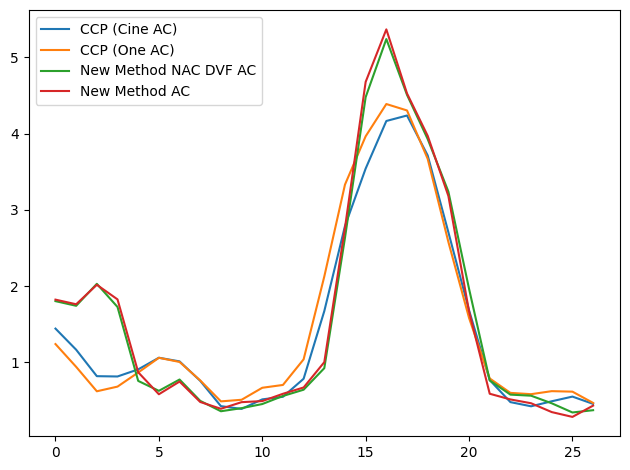
\includegraphics[width=1.0\linewidth]{figures/profile.png}
        
        % \vspace{-0.5cm}
        
        \captionsetup{singlelinecheck=false, justification=centering}
        \caption{A profile across the lesion for; ungated (CINE-\gls{CT}), ungated (static \gls{CT}), \gls{NAC} \gls{MM}, \gls{AC} \gls{MM}.}
        
        \label{fig:profile}
        % \vspace{-0.5cm}
    \end{figure}
    
    \begin{table}
        % \vspace{-0.0cm}
        \centering
        
        \captionsetup{singlelinecheck=false, justification=centering}
        \caption{Comparison of \gls{SUV}\textsubscript{max}, \gls{SUV}\textsubscript{median} and \gls{SUV}\textsubscript{peak} between; ungated (CINE-\gls{CT}), ungated (static \gls{CT}), \gls{NAC} \gls{MM}, \gls{AC} \gls{MM}.}
        
        % \vspace{-0.0cm}
        
        \resizebox*{0.8\linewidth}{!}
        {
            \begin{tabular}{||c|ccc||}
                \hline
                \textbf{\gls{SUV}} & \textbf{Max} & \textbf{Median} & \textbf{Peak} \\
                \hline
                \textbf{Ungated (CINE-\gls{CT})}    & $4.63$ & $2.73$ & $3.39$ \\
                \textbf{Ungated (static \gls{CT})}  & $4.66$ & $3.05$ & $3.54$ \\
                \hline
                \textbf{\gls{NAC} \gls{MM}}         & $5.56$ & $3.18$ & $4.07$ \\
                \textbf{\gls{AC} \gls{MM}}          & $5.43$ & $3.18$ & $4.00$ \\
                \hline
            \end{tabular}
        }
        
        \label{tab:suv}
        % \vspace{-0.5cm}
    \end{table}
    
     The ungated and the \gls{MM} data can be seen in~\Fref{fig:visual_analysis}. When compared visually structures can be seen, less blurred, in the \gls{MM} data that cannot be seen in the ungated data, for instance, structures at the boundary between the diaphragm and the lung. The different levels of blurring in the ungated (CINE-\gls{CT}) and static \gls{CT} could be attributed to the constraint put on the reconstruction by having a sharp \gls{Mu-Map} in one respiratory position in the static \gls{CT} case. Additionally the lesion itself can be seen to be more homogeneous, this can be observed in the profile across the lesion in~\Fref{fig:profile}. \gls{SUV} results can be seen in~\Fref{tab:suv} and consistently show that \glss{SUV} are greater for the \gls{MM} over the ungated method.

% \vspace{-0.5cm}

\section{Discussion and Conclusions} \label{sec:discussion_and_conclusions}
    Results from both a visual analysis, a comparison of profiles and \glss{SUV} show that the \gls{MM} provides volumes more free from blurring and less susceptible to artefacts when compared to the ungated data. Results also indicate that the \gls{NAC} \gls{MM} provides similar volumes while not requiring the additional computation of the \gls{AC} \gls{MM}.
    
    In the future, we will incorporate the estimated \glss{DVF} into the reconstruction. We will also compare more complex methods of combining motion estimation and image reconstruction based on \cite{Bousse2016b}. We also hope to find better results from improvements to \gls{TOF} resolution~\cite{Efthimiou2020UseScanners, Efthimiou2020TOF-PETBGO}.
    